\documentclass[12pt]{article}

\usepackage{amsmath,amsfonts,amssymb}
\usepackage[margin = 1in]{geometry}
\usepackage[none]{hyphenat}
\usepackage{fancyhdr}
\usepackage{graphicx}
\usepackage{float}
\usepackage{comment}
\usepackage{amsthm}
\usepackage{multicol}

\newcommand{\R}{\mathbb{R}}
\newcommand{\C}{\mathbb{C}}
\newcommand{\N}{\mathbb{N}}
\newcommand{\norm}[1]{\left\lVert#1\right\rVert}
\newtheorem{theorem}{Theorem}

\begin{document}

\begin{titlepage}
\begin{center}
\vspace*{1cm}
\huge{\textbf{MATH 680 Final Project}}\\
\vfill
\line(1,0){500}\\[1mm]
\huge{\textbf{PCA and its Variants}}\\
\line(1,0){500}\\
\vfill
Presented to Archer Y. Yang
\vfill
By Kevin Constantineau\\
Student ID: 260926167 \\
\today\\
\end{center}
\end{titlepage}

\section{Introduction}
The study of large datasets is integral to current day research. Examples include a biologist studying genotypes across a population or an investor trying to predict which stock will be beneficial for them. Most of the time, each data point depends on a large number of parameters and therefore it can be hard to find patterns. In this end of semester project, we present a grounds up approach to Principal Component Analysis (PCA) and a few of its key variants. More precisely, we showcase PCA, kPCA, PCA+, and PCA++, and reproduce the figures appearing in \cite{wu2025pcauniformityinducesrobustness}. Each of them will solve the problem of reducing the dimension of the data in an optimal way. Once the dimension has been reduced, large scale patterns can be witnessed by the naked eye. In a more general context, dimension reduction can be used to then allow a neural network to learn an high accuracy \textbf{linear} classifier.

Important note, if you wish to reproduce the figures yourself or verify the source code, it can all be found in the Final Project folder of \cite{Constantineau_MATH_680_Code}.


\section{PCA} \label{sec: PCA}
In this section, we present the original PCA algorithm. To being, we present the following problem. Suppose you have a large dataset of $N \in \N^+$ items that are characterized by $p \in \N^+$ features. You can therefore represent every item by a vector $x_n \in \R^p$. If $p$ is small ($\leq 3$), you could simply plot your data in $\R^p$ and visualize any emerging patterns. The problem arrises when $p$ is large. In this case, it can be very hard to get an understanding of what is going on.

We therefore try to leverage our intuitive understanding of lower dimensional plots to our advantage. To do this, we want to get an accurate lower dimensional representation of our data. Let $d \leq p$ and $f:\R^p \to \R^d$ be an encoder which takes our large dimensional data and sends it into a lower dimensional space. We also define $g:\R^d \to \R^p$, a decoder which takes the encoded data and sends it back to the high dimensional space. The goal is to make $f$ and $g$ as good as possible, ie we want $f,g$ to minimize
\[
    \frac{1}{N} \sum_{n = 1}^{N} \norm{x_n - g(f(x_n))}^2.
\]
In general, a problem of this form is difficult to solve, because we are minimizing functions. So instead, PCA focuses on a linear encoder / decoder of the form
\[
    f(x) = \begin{pmatrix}
        b_1^T \\
        \vdots \\
        b_d^T
    \end{pmatrix}x, 
    \quad g(z) = \sum_{j = 1}^{d}b_j z_j
\]
for some vectors $b_1, \dots, b_d \in \R^p$ with $\norm{b_j}=1$. Furthermore, we assume each feature of our dataset has mean 0. Recall that for a unit vector $v$, the projection of another vector $u$ onto $v$ is
\[
vv^Tu.
\]
Hence $g \circ f$ projects of our original data on the linear subspace spanned by the set of vectors $b_1, \dots, b_d$. Note that this subspace has dimension $\le d$ and the equality is achieved if and only if the vectors are linearly independent. We assume an even stronger condition, that the set of vectors is orthonormal. Note that this assumption is not restrictive. Given a basis for a d-dimensional vector space, you can always obtain an orthonormal basis for the same set. Going back to the minimization problem and plugging in our new representation of $f, g$ we obtain
\[
    \frac{1}{N} \sum_{n = 1}^{N} \norm{x_n - BB^Tx_n}
\]
where $B = (b_1, \dots, b_d)^T$. Then we see that
\[
\frac{1}{N} \sum_{n = 1}^{N} \norm{x_n - BB^Tx_n} = \frac{1}{N} \sum_{n = 1}^{N} \norm{x_n}- tr(B^T S B),
\]
where
\[
S = \frac{1}{N} \sum_{n = 1}^{N} x_n x_n^T = \frac{1}{N} X^T X, \quad X = \begin{pmatrix}
    x_1^T\\
    \vdots \\ 
    x_N^T\\
\end{pmatrix}.
\]
Therefore we equivalently have to maximize
\[
tr(B^T S B),
\]
Notice that $S$ is symmetric positive semi-definite as
\[
u^TSu = u^T \frac{1}{N} X^T X u = \frac{1}{N} (Xu)^T(Xu) = \frac{1}{N} \norm{Xu}^2 \ge 0.
\]
So the solution to our minimization problem is $B$ having columns equal to the eigenvectors of $S$ correspondong to the $d$ largest eigenvalues. These are indeed orthogonal since $S$ is symmetric. What we have now accomplished is reduced the dimension of original data in a way kept the maximum amount of information. Notice that in our projected space that is spanned by the columns of $B$, each item is a linear combination of those vectors. Therefore, we can plot our data using these coefficients.

It is also important to see that each eigenvalue of $S$ represents the variance captured along the linear subspace spanned by its corresponding eigenvector. This means that we can determine how much information was lost by summing up the remaining eigenvalues. In practice, we typically look for significant drop in the magnitude of the eigenvalues to determine the ``true" linear dimension of the data.

With the presentation of the method out of the way, we show an example where PCA can provide key insights on a data set that lives in a very high dimension. The example chosen in this case is from homework 1. We are given a subsection of length 10101 of 995 people's genome along with their sex and the population they belong to. These subsections can be written as words of length 10101 in the alphabet `A', `T', `C', `G'. Using this we can create a binary matrix $X$ which encodes when a specific individual's neucleodites differs from the population mode for that. More precisely $ x_{i,j} = (X)_{i,j} = 0$ when the $i$th individual's $j$th neucleobase matches the mode of the population's $j$ neucleodbase. Otherwise, we set $x_{i,j} = (X)_{i,j} = 1$. We now apply PCA with $d = 2,3$ and plot the labelled data in figure~\ref{fig: pca}.

\begin{figure}[H]
\centering
    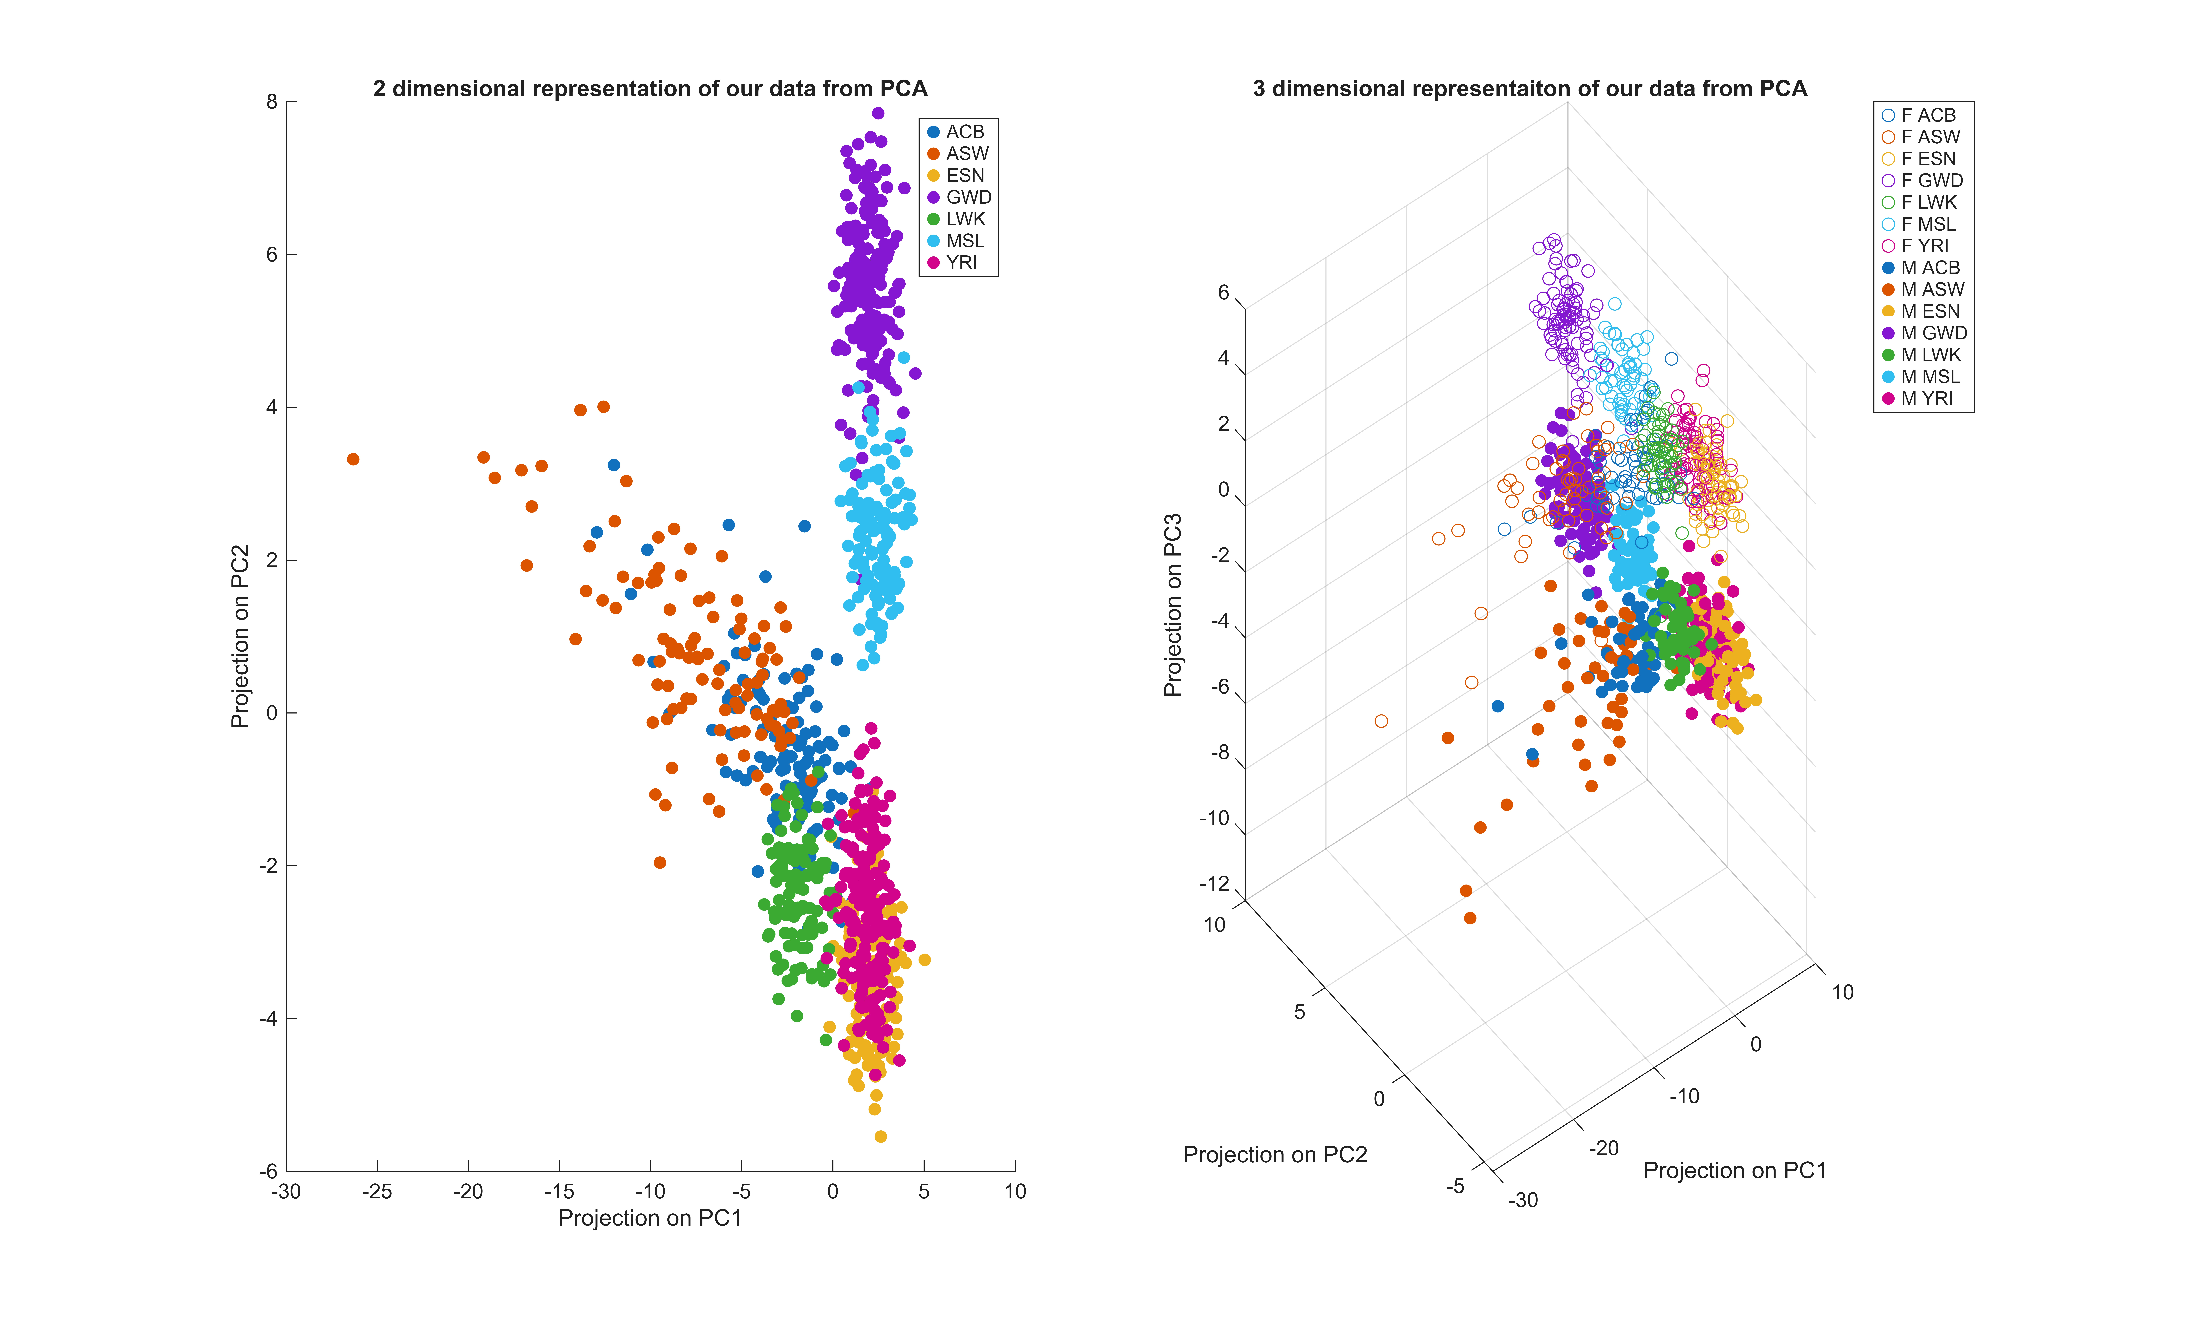
\includegraphics[width=0.8\textwidth]{Figures/PCA.pdf}
    \caption{\textbf{Left/Right:} Projection of the data on the first two/three principal components using PCA.}
\label{fig: pca}
\end{figure}

We see that in the case $d=2$, PCA is able to make apparent a pattern in the gneome of each population. When $d=3$, we see that the third principal component mostly captures differences in sex.

\section{kPCA} \label{sec: kPCA}
Now that we have shown the strengths of PCA, we note its weakness: Its linear nature. Since PCA remains a linear method, it is unable to capture nonlinear dimension and more complex structures. This is where kernel PCA (kPCA) comes in. The idea is to augment our data into a higher dimensional space in a way that it becomes linearly separable and then apply PCA in that new space. More precisely, we consider a nonlinear map $\phi:\R^p \to \R^P$ with $P \ge p$ and apply PCA on the new dataset $\phi(x_n)$. So now we define 
\[
X = \begin{pmatrix}
    \phi(x_1)^T \\
    \vdots \\
    \phi(x_n)
\end{pmatrix}
\]
to be our new data matrix. Note that even if the original data is centered, nothing is ensuring that the augmented data is. The fix consists of multiplying by a centering matrix and doesn't change the method, so we move along assuming the new data is centered. Applying PCA to the data matrix $X$ is going to find the $d$ largest eigenvalues and assosicated eigenvectors of the matrix
\[
C = \frac{1}{N} \sum_{n = 1}^{N} \phi(x_n)\phi(x_n)^T.
\]
In practice, $\phi$ might be a complicated map the goes into a much higher dimension, leading to long computations. Let us now see how we can avoid ever having to compute it. The eigen problem is 
\[
C b_j = \lambda_j b_j \iff \frac{1}{N}\sum_{n = 1}^{N} \phi(x_n)\phi(x_n)^T b_j = \lambda_j b_j.
\]
Letting $c_{j,n} = \frac{1}{N\lambda_j}\phi(x_n)^T b_j$, we see that we can write 
\[
b_j = \sum_{n = 1}^{N} c_{j,n} \phi(x_n) ,
\]
so $b_j$ is a linear combination of our augmented data set. With this new expression for $b_j$, we return to the eigen problem above and obtain
\[
\frac{1}{N}\sum_{n = 1}^{N} \phi(x_n)\phi(x_n)^T \sum_{m = 1}^{N} c_{j,m} \phi(x_m) = \lambda_j \sum_{n = 1}^{N} c_{j,n} \phi(x_n).
\]
which we can rearrange into
\[
\frac{1}{N}\sum_{n = 1}^{N} \phi(x_n)\sum_{m = 1}^{N} c_{j,m} \phi(x_n)^T \phi(x_m) = \lambda_j \sum_{n = 1}^{N} c_{j,n} \phi(x_n).
\]
The key insight is now to realise thay this equation needs to hold when you multiply it on both sides by $\phi(x_\ell)^T$ for $l = 1, \dots, N$. This gives
\[
\frac{1}{N}\sum_{n = 1}^{N} \phi(x_\ell)^T\phi(x_n)\sum_{m = 1}^{N} c_{j,m} \phi(x_n)^T \phi(x_m) = \lambda_j \sum_{n = 1}^{N} c_{j,n} \phi(x_\ell)^T\phi(x_n).
\]
The important thing to notice is that this expression only depends on the inner product between two augmented points, and not the point themselves. So we define the $N \times N$ \textit{kernel matrix} $K$ element-wise by
\[
K_{n,m} = \phi(x_n)^T\phi(x_m).
\]
The above equation becomes
\[
\frac{1}{N}\sum_{n = 1}^{N} K_{\ell,n}\sum_{m = 1}^{N} c_{j,m} K_{n,m} = \lambda_j \sum_{n = 1}^{N} c_{j,n} K_{\ell,n},
\]
or
\[
K^2 c_j = N \lambda_j K c_j,
\]
in matrix form. We remove a factor of $K$ on each side to obtain the eigen problem on the matrix $K$. So the solution is $c_1, \dots, c_d$ to be the eigenvectors associated to the $d$ largest eigenvalues of $K$. The last step is to get the correct norm of $c_j$ such that $\norm{b_j} = 1$.
\[
\begin{split}
    \norm{b_j}^2 = b_j^T b_j &= \left(\sum_{n = 1}^{N} c_{j,n} \phi(x_n)^T \right) \left(\sum_{n = 1}^{N} c_{j,n} \phi(x_n)\right) \\
    &= \sum_{n = 1}^{N} \sum_{m = 1}^{N} c_{j,n}c_{j,m} \phi(x_n)^T \phi(x_m) \\
    &= \sum_{n = 1}^{N} c_{j,n} \sum_{m = 1}^{N} K_{n,m} c_{j,m} \\
    &= c_j^T K c_j \\
    &= N \lambda_j \norm{c_j}^2.
\end{split}
\]
So we need to ensure $\norm{c_j} = \frac{1}{\sqrt{N \lambda_j}}$. Recall that in PCA, we are really after the coefficients of the projection, more precisely
\[
z_{j,n} = b_j^T \phi(x_n) = \sum_{m = 1}^{N} c_{j,m} K_{m,n}.
\]
We've also seen in class that any positive semi definite kernel matrix corresponds to a given transformation $\phi$ and vice versa. Therefore, we typically choose a kernel function $k$ rather than choose a transformation $phi$ if we don't know apriori what the nonlinear structure is.

With the method now presented, we showcase an example of kPCA. We build our own dataset with a clear nonlinear structure, where the red points are near the origin, and the blue dots are further. We then apply PCA and kPCA with $d = 2$ and show the results in figure~\ref{fig: kpca}. The chosen kernel function is the Gaussian RBF kernel
\[
k(x,y) = e^{-\frac{1}{2}\norm{x-y}^2},
\]
which does generate a positive semi definite kernel matrix. One can see that, as expected, PCA does not lead to a space where the red and blue dots can be linearly separated. However, the nonlinear aspect of kPCA clearly allows a linear classifier to classify the red and blue dots.

\begin{figure}[H]
\centering
    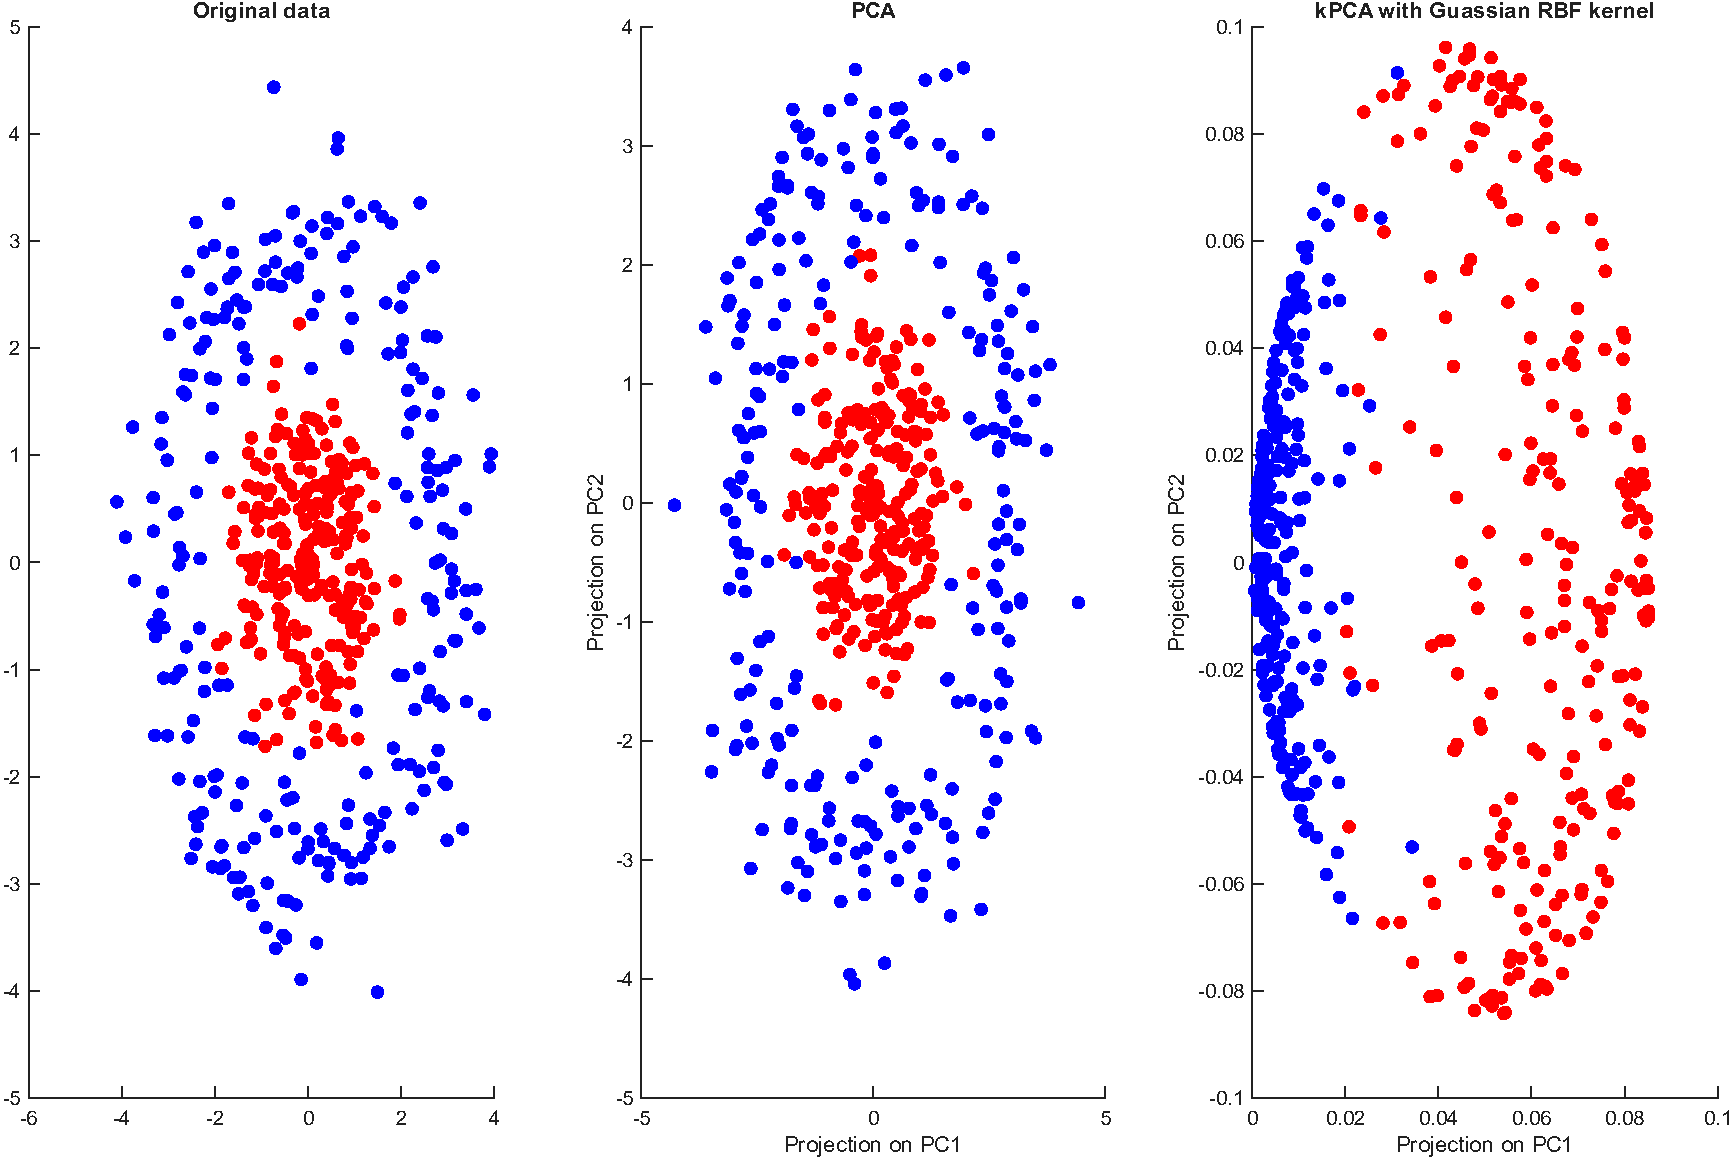
\includegraphics[width=0.8\textwidth]{Figures/kPCA.pdf}
    \caption{\textbf{Left:} The original 2-dimeisonal dataset with nonlinear structure \textbf{Middle/Right:} 2-dimensional representation of the data after applying PCA/kPCA.}
\label{fig: kpca}
\end{figure}

\section{PCA+} \label{sec: PCA+}
In this section, we introduce PCA+, a contrastive appraoch to regular PCA. This contrastive approach will allow these PCA+ to correctly filter out background noise and only focus on the ``core" structure of the problem. The method presented in this section will be taken from section~() of \cite{wu2025pcauniformityinducesrobustness}. For this section, we assume we have paired data $\{ x_n, x_n+\}_{n = 1}^{N}$ in $\R^p$ which can be decomposed into a shared signal, an independent background, and noise:
\[
x_n = A w_n + B h_n + \varepsilon_n, \quad
x_n^+ = A w_n + B h'_n + \varepsilon'_n, \quad
\forall n = 1, \dots, N,
\]
where $A \in \R^{p \times k}$ and $B \in \R^{p \times m}$ have orthogonal columns spanning the signal and background subspaces, respectively. Furhtermore, $w_n \in \R^k$, $h_n, h'_n \in \R^m$ are the shared signal factor and independent background factors. Lastly, $\varepsilon_n, \varepsilon'_n \in \R^p$ are the independent background noise. Given the presentation of $A,B$, we can write them as
\[
A = \left( \sqrt{\lambda_{A,1}} \nu_{A,1}, \dots, \sqrt{\lambda_{A, k}} \nu_{A, k} \right), \quad B = \left( \sqrt{\lambda_{B,1}} \nu_{B,1}, \dots, \sqrt{\lambda_{B, m}} \nu_{B, m} \right),
\]
where each $\nu_{A,i}, \nu_{B,j}$ are unit vectors representing the principal direction with variance $\lambda_{A,i}, \lambda_{B,j}$, respectively. The idea behind the method is to contrast pairs $(x_n x_n^+)$ that share the same signal $A w_n$ but differ in background and noise in order to isolate the shared signal and obtain some low dimensional information related to it. The paper [] further imposes 3 conditions on the data. Those being
\begin{enumerate}
    \item The column spaces of the signal and background matrices are mutually orthonal, ie $\text{span}(A) \perp \text{span}(B)$. 
    \item $w_n \sim \mathcal{N}(0, I_k)$, $h_n, h'_n \sim \mathcal{N}(0, I_m)$ all independent.
    \item $\varepsilon_n, \varepsilon'_n \sim \mathcal{N}(0, I_p)$ independent.
\end{enumerate}
As [] mentions, these assumptions are there to simplify the analysis of the problem but the method remains robust to violations. Consider a contrastive loss composed of an alignemnt term and a uniformity term for an encoder $f: \R^p \to \R^d$
\[
\mathcal{L}_{constrastive} = - \mathbb{E}_{(x,x^+)} \left[f(x)^Tf(x^+)\right] + \tau \norm{\mathbb{E}_x\left[f(x)f(x)^T\right] - I_d}_F,
\]
where $\tau > 0$ is a paramter controlling the strength of uniformity. We focus on the case where $\tau = 0$, which means our method only enforces alignment of positive pairs and disregards uniformty. As in PCA, we look for a linear encoder that minimizes the alignment loss. This leads to the minimization problem
\[
\min -\frac{1}{N} \sum_{n = 1}^{N} \left(V^T x_n\right)^T \left(V^T x_N^+\right) \iff \max tr\left(\frac{1}{N} V^T X^T X^+ V\right),
\]
where as before $V \in \R^{p \times d}$ is an orthonormal matrix and $X, X^+ \in \R^{N \times p}$ are matrices whos rows are the data. We do not know that $X^T X^+$ is symmetric, so we artifically construct a symmetric matrix
\[
S^+ = \frac{1}{2N}(X^T X^+ + {X^+}^T X),
\]
which can be shown to satisfy $\mathbb{E}[S^+] = AA^T$ by the 3 assumptions of our data, exactly what we want. Indeed,
\[
X = W^T A^T + H^T B^T + E^T, \quad X^+ = W^T A^T + H'^T B^T + E'^T,
\]
where $W = (w_1, \dots, w_N)$, $H = (h_1, \dots, h_N)$, $E = (\varepsilon_1, \dots, \varepsilon_N)$, and similarly for $H', E'$. So then,
\[
\begin{split}
   2N S^+ &= X^TX^+ + {X^+}^TX \\
   &= (AW + BH + E)(W^T A^T + H'^T B^T + E'^T) + (AW + BH' + E')(W^TA^T + H^TB^T + E^T) \\
   &= 2AWW^TA^T + \Delta, 
\end{split}
\]
where
\[
\begin{split}
    \Delta = &AWH'^TB^T + AWE'^T + BHH'^TB^T + BHH^TB^T +BHE'^T + EW^TA + EH'^TB^T + EE'^T \\
    &+ AWH^TB^T + AWE'^t + BH'W^TA^T + BH'H^TB^T+BH'E^T + E'W^TA^T + E'H^TB^T + E'E^T.
\end{split}
\]
Notice that by the independance and zero mean assumption, we have that $\mathbb{E}[\Delta] = 0$ since each term only has 1 copy of $W,H,H',E,E'$, which all have expectation 0. With that in mind, we are left with
\[
\mathbb{E}[2NS^+] = \mathbb{E}[2AWW^TA^T] \iff \mathbb{E}[S^+] = AA^T,
\]
as we know $w_n \sim \mathbb{N}(0, I_k)$. So we now solve for orthonormal matrix $V$ that maximizes
\[
tr(V^T S^+ V),
\]
which is precisely PCA on $S^+$. Thus the solution is the columns of $V$ to be the $d$ eigenvectors corresponding to the $d$ largest eigenvalues of $S^+$. We know that as the population gets large enough, this will tend to solution to PCA on the shared signal data. As pointed out in \cite{wu2025pcauniformityinducesrobustness}, this algorithm performs well only if the background signal is weak in comparisson to the shared signal. More precisely, we need $\lambda_{A,d} >> \lambda_{B,1}$ or $N$ large enough so that $S^+ \approx AA^T$.

With the method now presented, we showcase its strength as opposed to regular PCA by building a dataset $X, X^+$ as outlined above with a significant background variance. We then plot the accuracy of PCA and PCA+ at recovering the original signal across different values of $N$ in figure~\ref{fig: pcap}. As in \cite{wu2025pcauniformityinducesrobustness}, we measure the estimation error but measuring the sine of largest principal angle between $A$ and $V$. As the figure shows, PCA+ is able to accurately recover the original signal as $N$ grows large. Meanwhile, PCA is unable to recover it at all for all $N$.

\begin{figure}[H]
\centering
    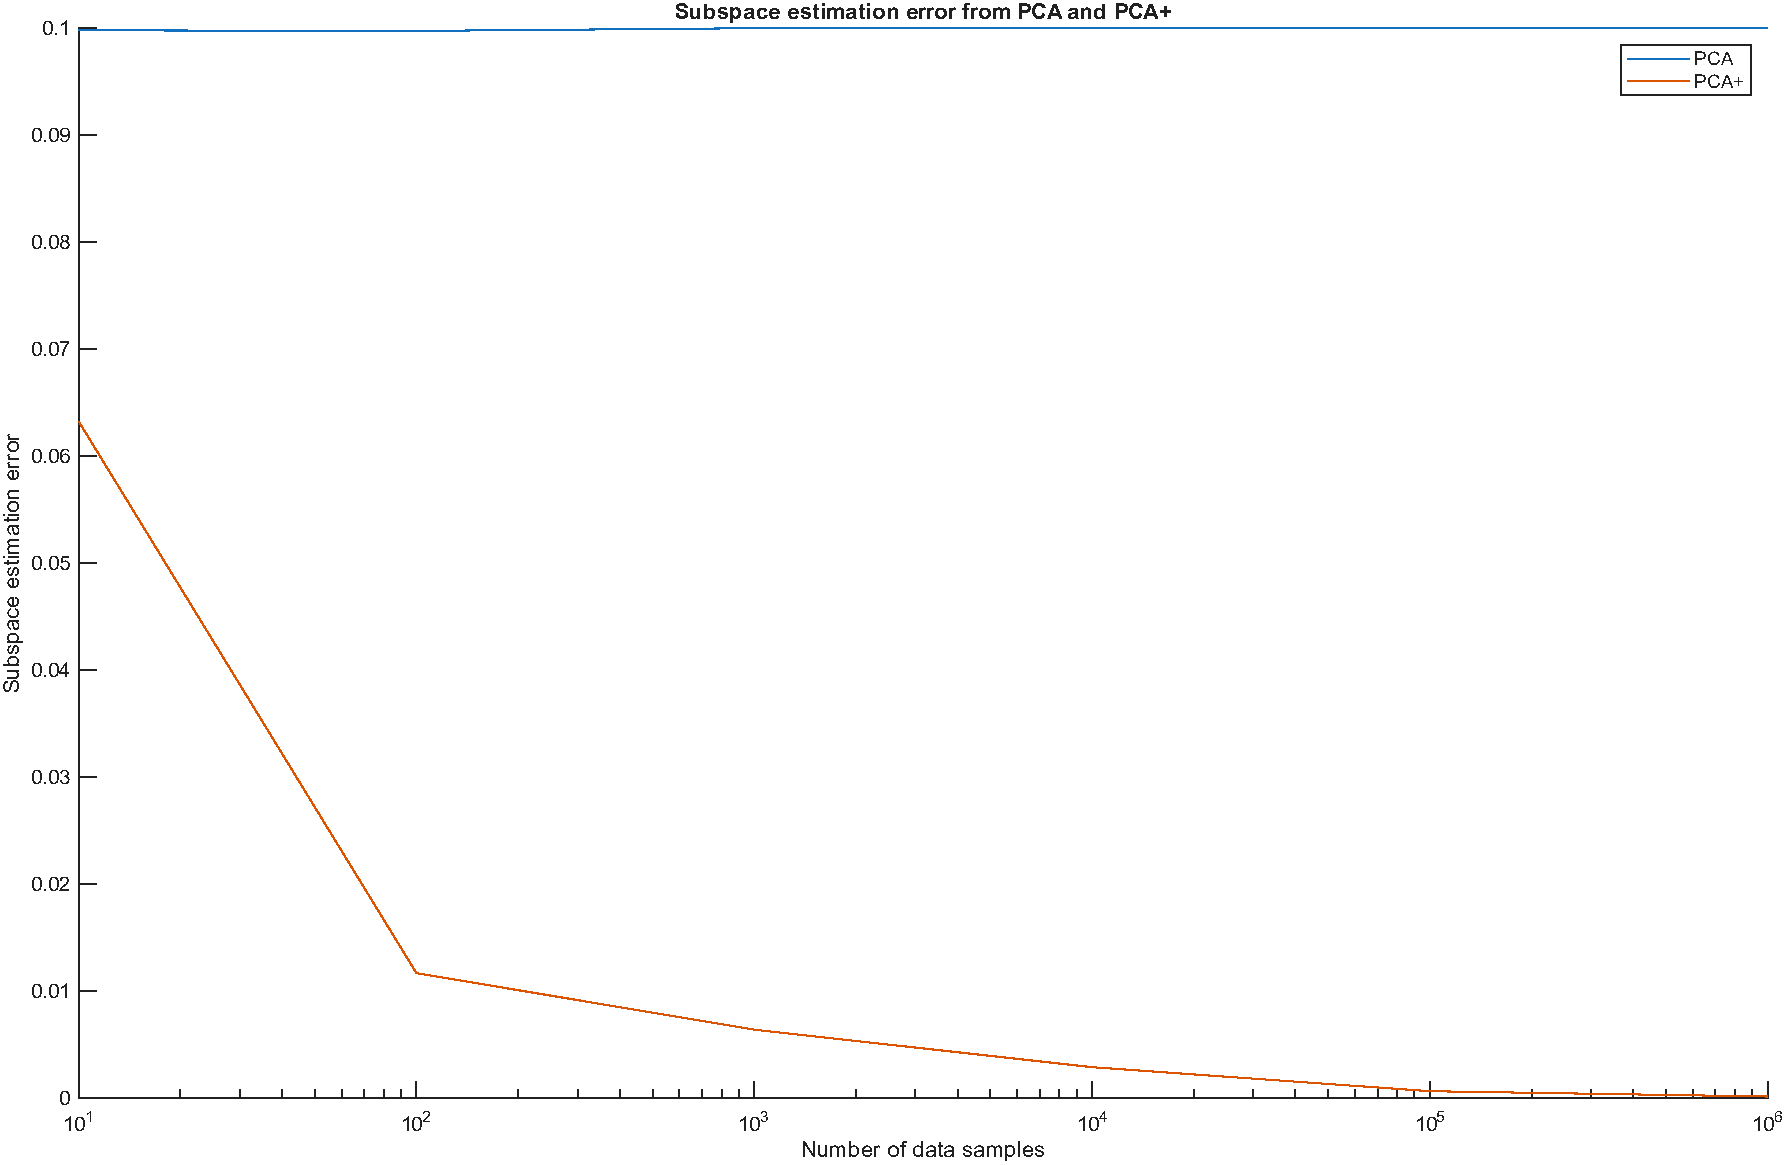
\includegraphics[width=0.8\textwidth]{Figures/PCAp.pdf}
    \caption{Comparing the efficacy of PCA and PCA+ on an artificial paired dataset of varying sizes.}
\label{fig: pcap}
\end{figure}

\section{PCA++}
In this section, we present a more powerful version of PCA+ better handled to deal with very high strength background noise. This method will be taken from section~() of \cite{wu2025pcauniformityinducesrobustness}. The key idea is to not ignore the uniformity term from contrastive loss. Instead, we impose that the projected features are uniformly distributed while minimzing the alignment loss. We assume the same setup of paired data as PCA+ and maximize
\[
tr(V^TS^+V) \quad \text{such that} \quad V^TSV = I_d, 
\]
where $V \in \R^{p \times k}$, $S^+ = \frac{1}{2N} (X^T X^+ + {X^+}^T X)$ and $S = \frac{1}{N} X^TX$. Notice that the constraint enforces
\[
V^TSV = \frac{1}{N} \sum_{n=1}^{N} (Vx_n)(Vx_n)^T = I_d,
\]
which corresponds to the uniformity loss being 0 in the contrastive loss. The paper shows that the problem is equivalent to solving the generalized eigenvalue problem
\[
S^+v_j = \lambda_jSv_j \quad \forall j = 1, \dots, p.
\]
As with PCA and PCA+, the solution is $V$ having columns equal to eigenvectors corresponding to the top $d$ generalized eigenvalues. For implementation details, the paper provides an algorithm that solves this problem in their appendix. Now in pracitce, when the dimension is very high, $S$ can be ill-conditioned. This makes solving the generalized eigenproblem numerically unstable. To help this, we replace $S$ by its rank $s$ approximation $S_s$ and solve
\[
S^+v_j = \lambda_jS_sv_j \quad \forall j = 1, \dots, p.
\]
By construction, $S_s$ is well conditioned so there is no issue. This corresponds to enforcing uniformity only in the directions which already represent the largest variation and are therefore less likely to be due to noise.

When analysis the error of PCA++, there are 2 different regimes \cite{wu2025pcauniformityinducesrobustness} considered. The first being that $\lambda_{A,i}, \lambda_{B_j} \ge c = \frac{p}{N}$. This means that the variance should be detectable. They refer to this as the detectable spike regime. The second is the growing spike regime, where $N,p, \lambda_{A,i} \lambda_{B,j} \to \infty$ in such a way that
\[
\frac{p}{N \lambda_{A,i}} \to c_{A,i} , \quad \frac{p}{N \lambda_{B,j}} \to c_{B,j}.
\]
This is the growing spike regime.

In the detectable spike regime, we expect the square of the $d$-dimensional subspace estimation error of PCA++ to converge to
\[
1 - \frac{1 - c {\lambda_{A,d}}}{1 + c\frac{1}{\lambda_{A,d}}},
\]
as $N,p \to \infty$ maintaining $\frac{p}{N} = c$. Meanwhile, in the growing spike regime, we expect the square of the $d$-dimensional subspace estimation error of PCA++ to converge to
\[
\frac{c_{A,d}}{1+c_{A,d}}.
\]
 
To put everything to the test, we consider a simple example where $A = (1, 0, \dots, 0)$ and $B = (0,1,0, \dots, 0)$. The following plots will all be generated from this example. We begin by comparing the performance of PCA, PCA+, and PCA++ on this example for varying aspect ratios ($p/N$) and relative strength between $A$ and $B$ ($\lambda_{A,1}/\sqrt{\lambda_{B,1}}$). The results can be found in figure~\ref{fig: overview}, a reproduction of figure 1 from \cite{wu2025pcauniformityinducesrobustness}.

\begin{figure}[H]
\centering
    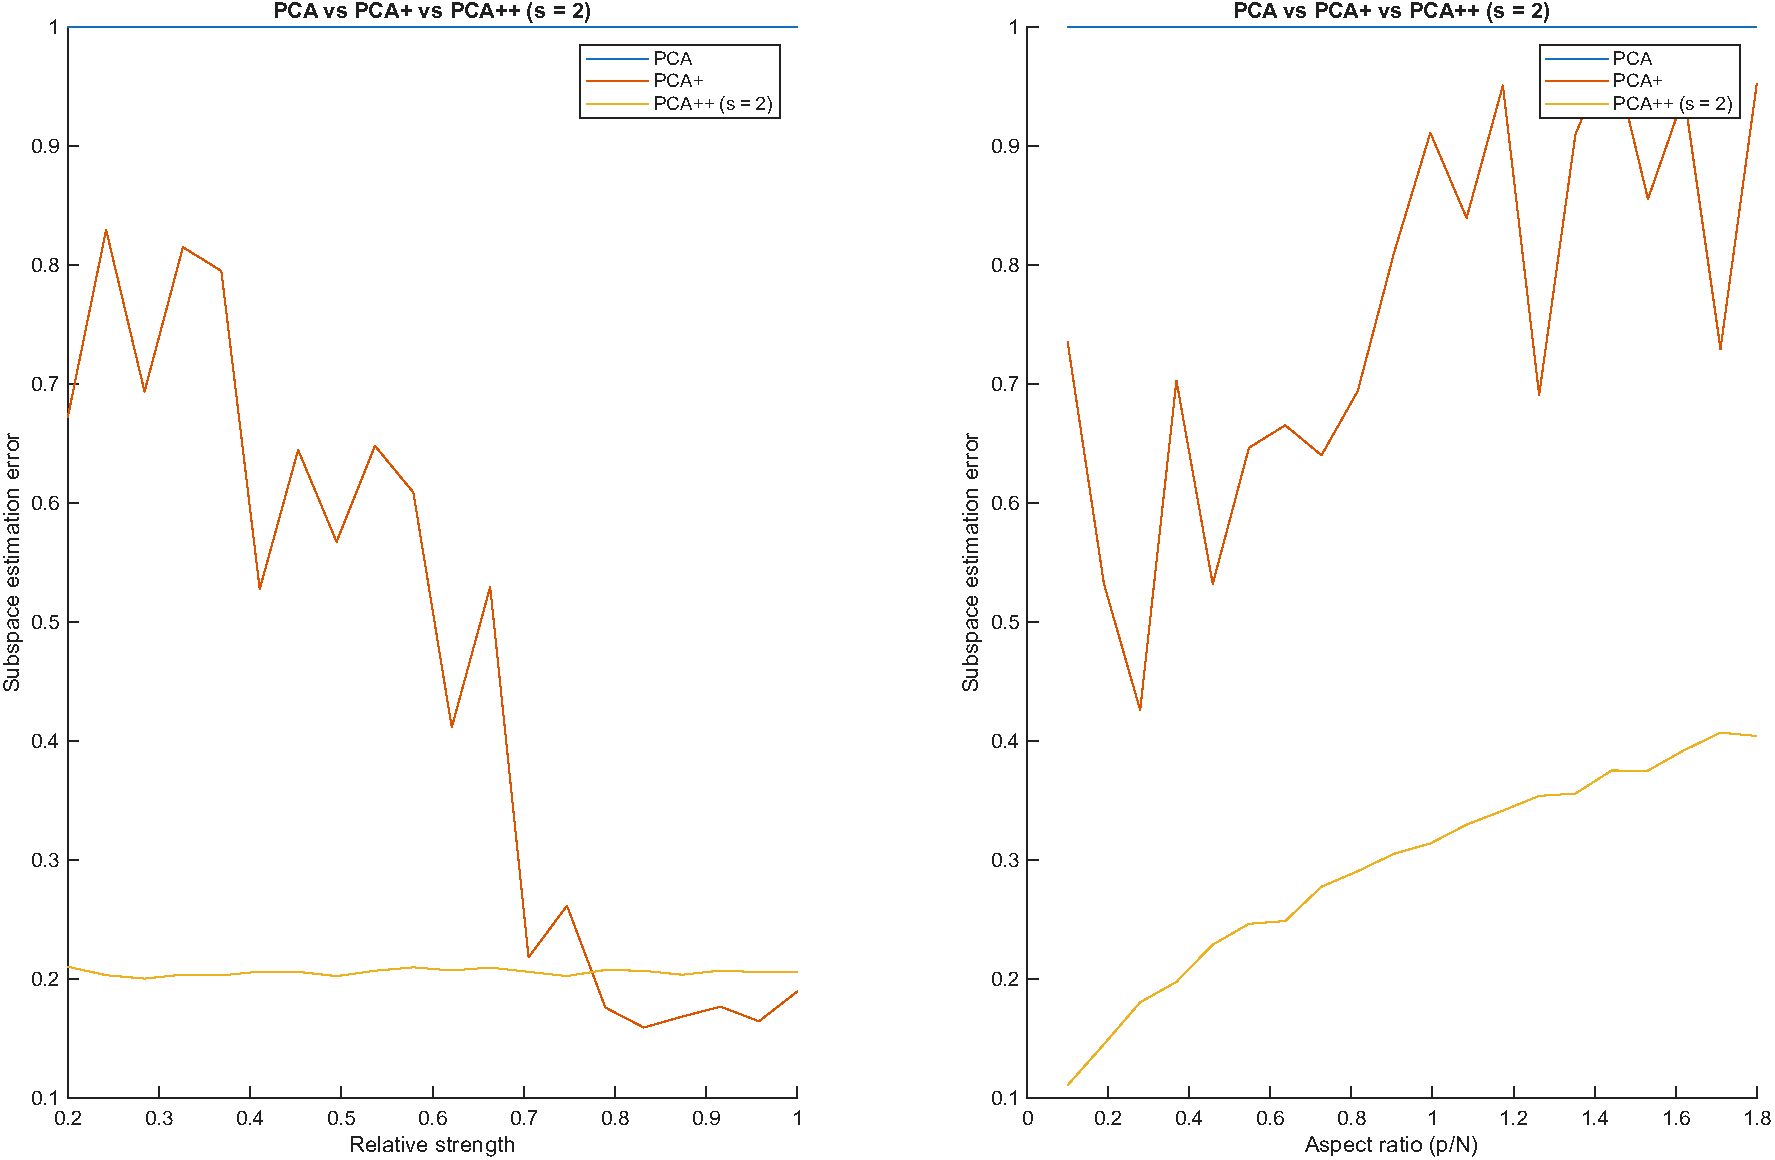
\includegraphics[width=0.8\textwidth]{Figures/PCApp.pdf}
    \caption{\textbf{Left:} Comparing the performance of PCA, PCA+, and PCA++ ($s=2$) on the simple example for varying relative strength between the shared and background signals. \textbf{Right:} Comparing the performance of PCA, PCA+, and PCA++ ($s=2$) in the same example varying the aspect ratio.}
\label{fig: overview}
\end{figure}

One can see that PCA performs terribly in all tested cases and PCA++ performs the best or similarly to PCA+. What is more impressive is that PCA++ does not deterioate as the background signal increase in strength, as opposed to PCA+. Next, we reproduce figure 2 which captures the usefulness of truncating PCA++ with figure~\ref{fig: pcapp_truncations}.

\begin{figure}[H]
\centering
    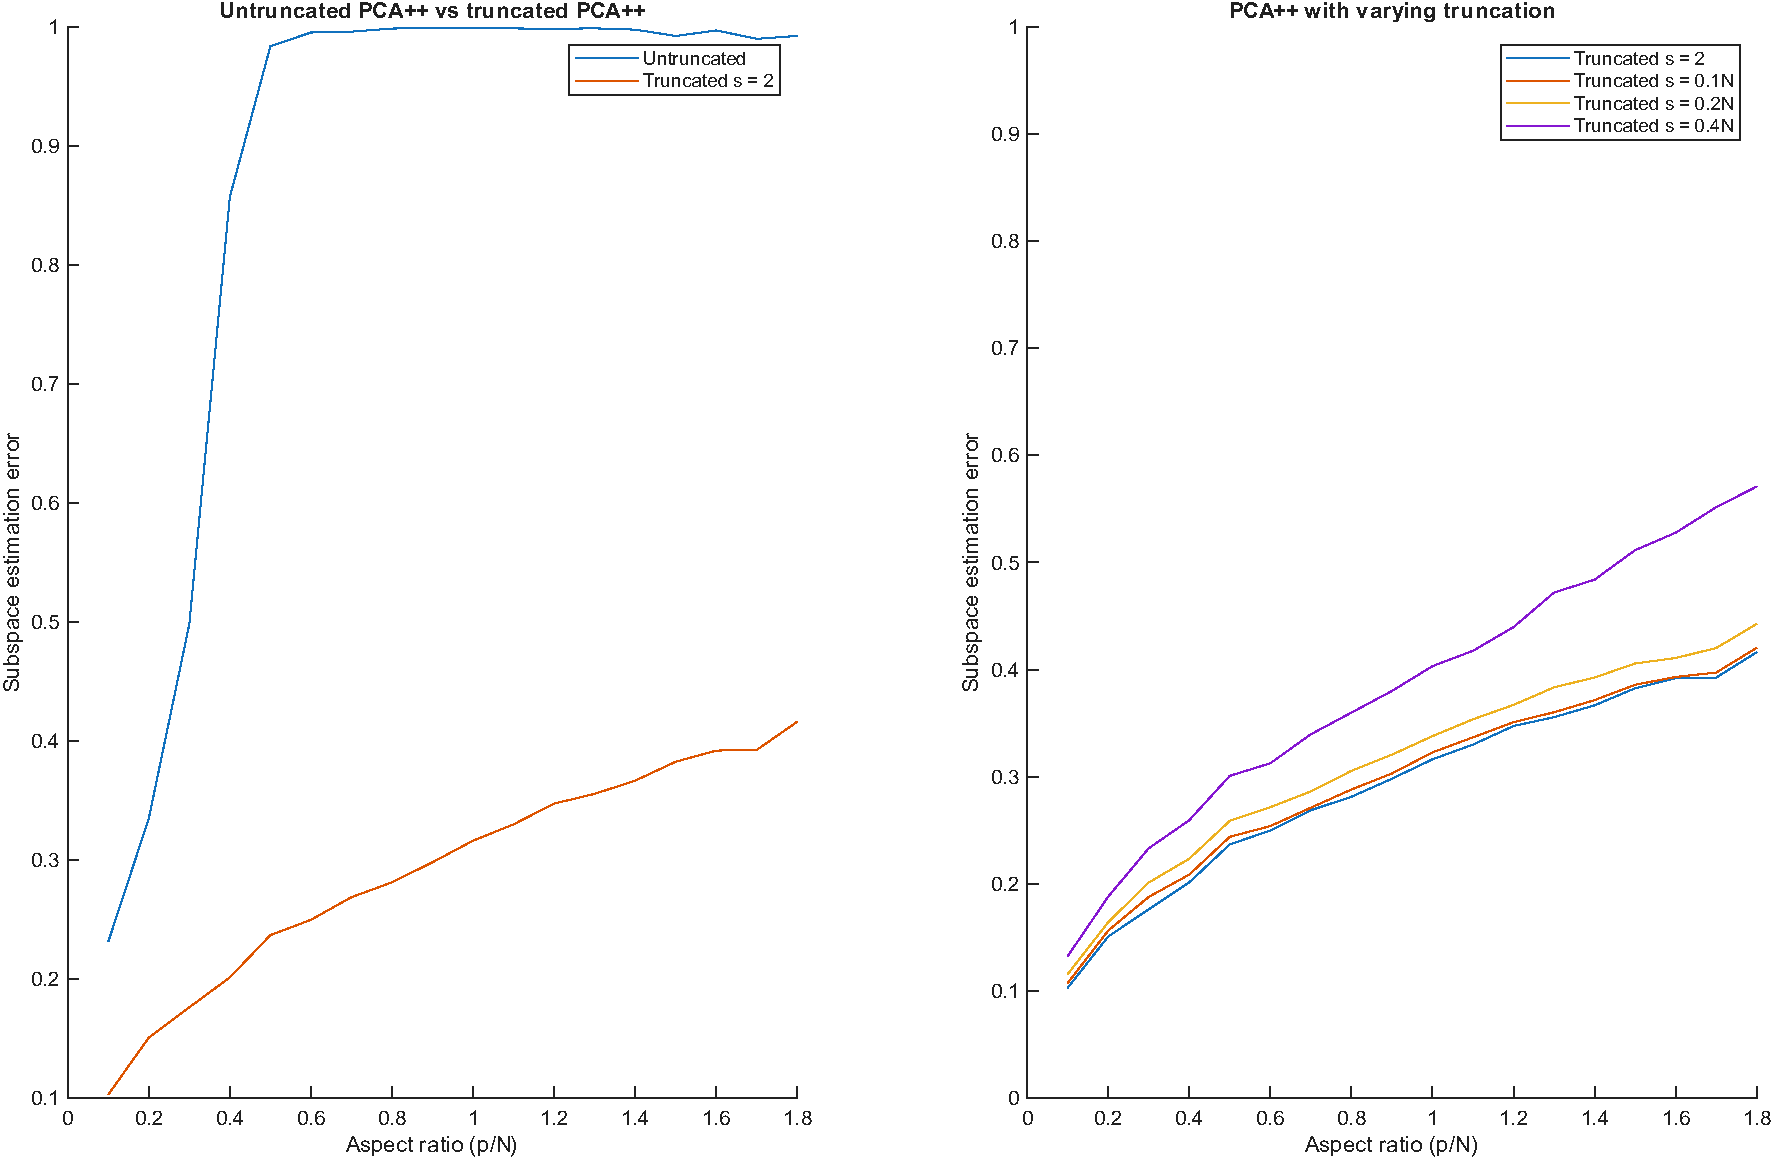
\includegraphics[width=0.8\textwidth]{Figures/PCApp_truncations.pdf}
    \caption{\textbf{Left:} Comparing the performance of untruncated PCA++ and truncated PCA++ ($s=2$) as we vary the aspect ratio. \textbf{Right:} Comparing the performane of different truncations of PCA++ as we vary the aspect ratio.}
\label{fig: pcapp_truncations}
\end{figure}

We see from the result that truncation has a massive effect on the accuracy of PCA++ as the aspect ratio increases. At around an aspect ratio of $0.5$, untruncated PCA++ diverges completely, while truncated PCA++ deteriorates steadily. From the right figure, we see that a sharpher truncation was best, with $s=2$ and $s=0.1N$ being very close to one another. The next figure we recreate is figure 3, which shows that truncated PCA++ ($s=10$) accurately follows the estimated error bounds in the detectable and growing spike regimes.

\begin{figure}[H]
\centering
    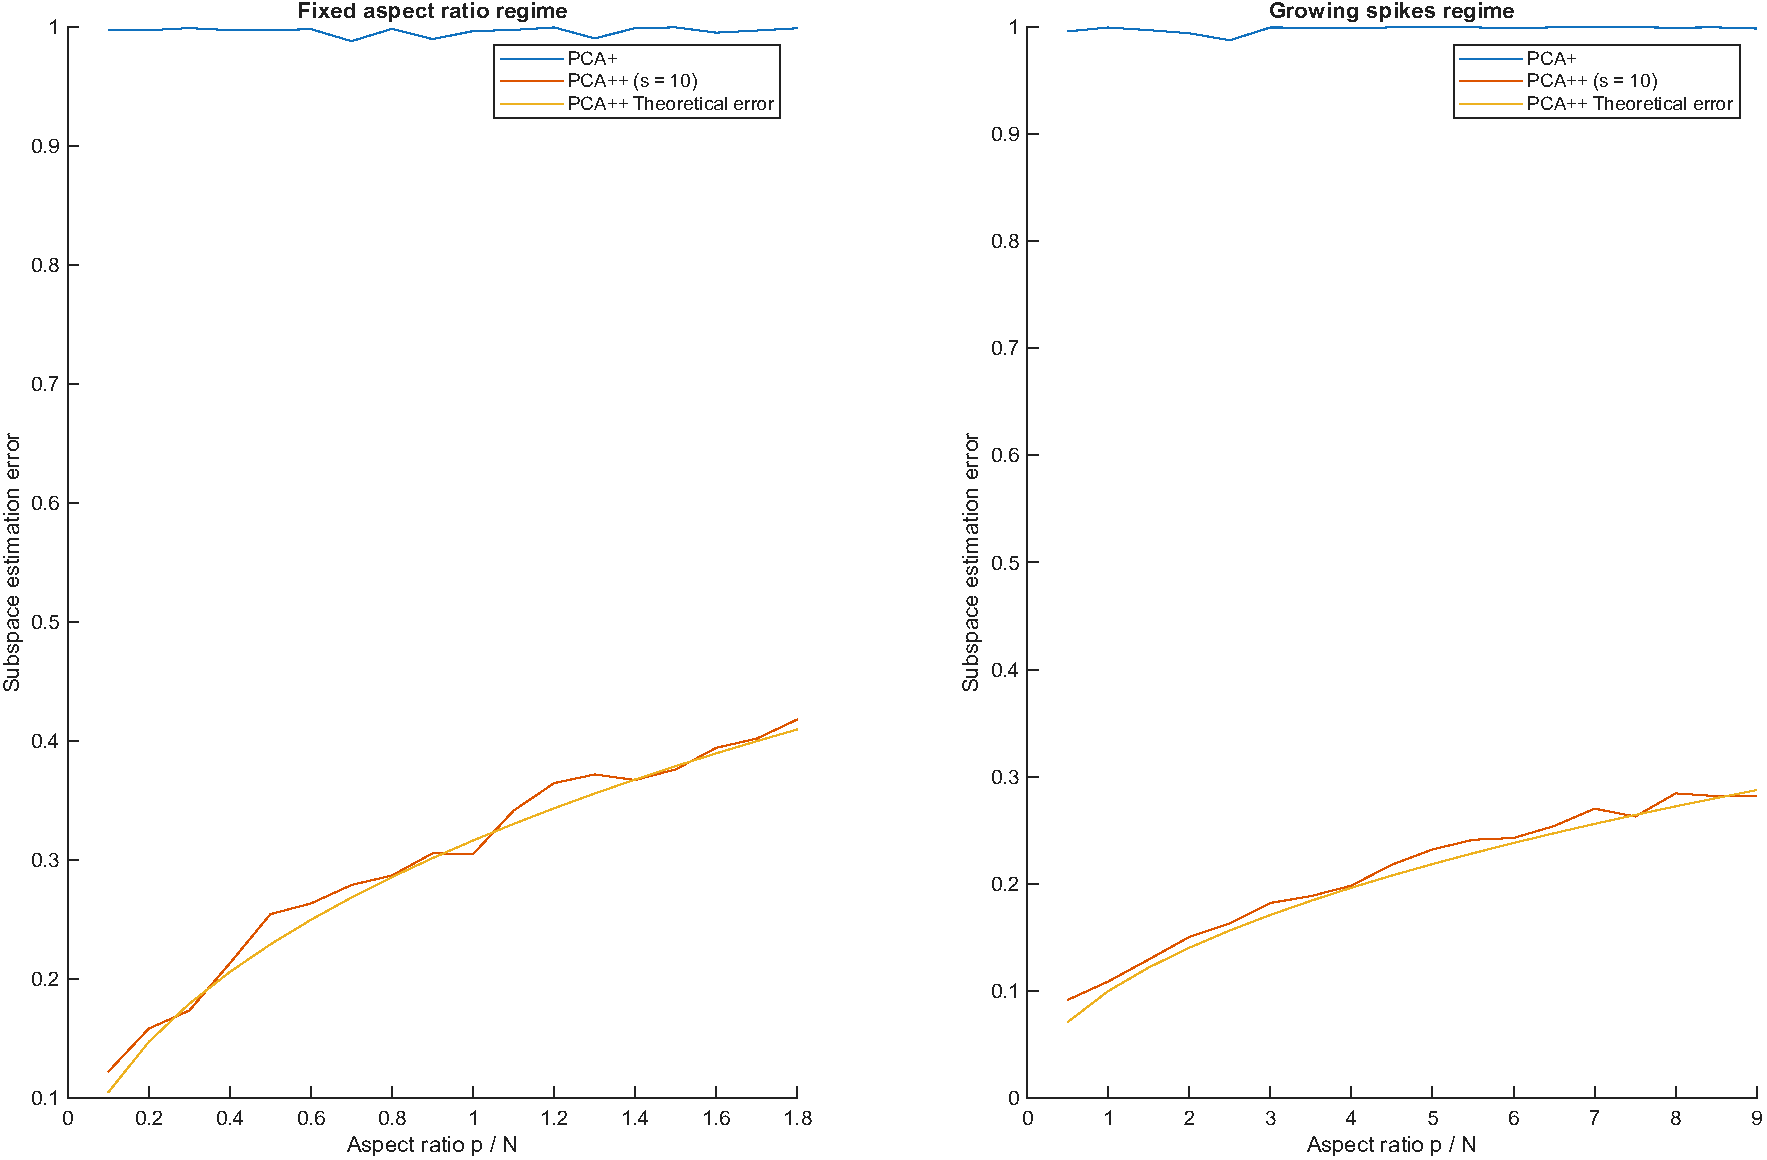
\includegraphics[width=0.8\textwidth]{Figures/theory.pdf}
    \caption{\textbf{Left/Right:} Comparing the performance of truncated PCA++ ($s=10$) in the detectable/growing spike regimes to the predicted error and PCA+.}
\label{fig: theory}
\end{figure}

As seen in figure~\ref{fig: theory}, PCA++ follows closely its predicted error bound. In practice, we simulated the growing spike regime by multiplying both $\lambda_{A,1}, \lambda_{B,1}$ and $p$ by 5.

\section{MNIST Dataset}
Finally, we reproduce figure 4 which applies PCA++ to a real world example: the MNIST digit dataset. To put us into context, we know that PCA alone can reliably differentiate the `0' and `1' digits. Now we will take these digits and superimpose them with a powerful background noise to create a dataset of 10000 pairs. We then apply PCA, PCA+, and PCA++ ($s=10$) and see how they each fair.

\begin{figure}[H]
\centering
    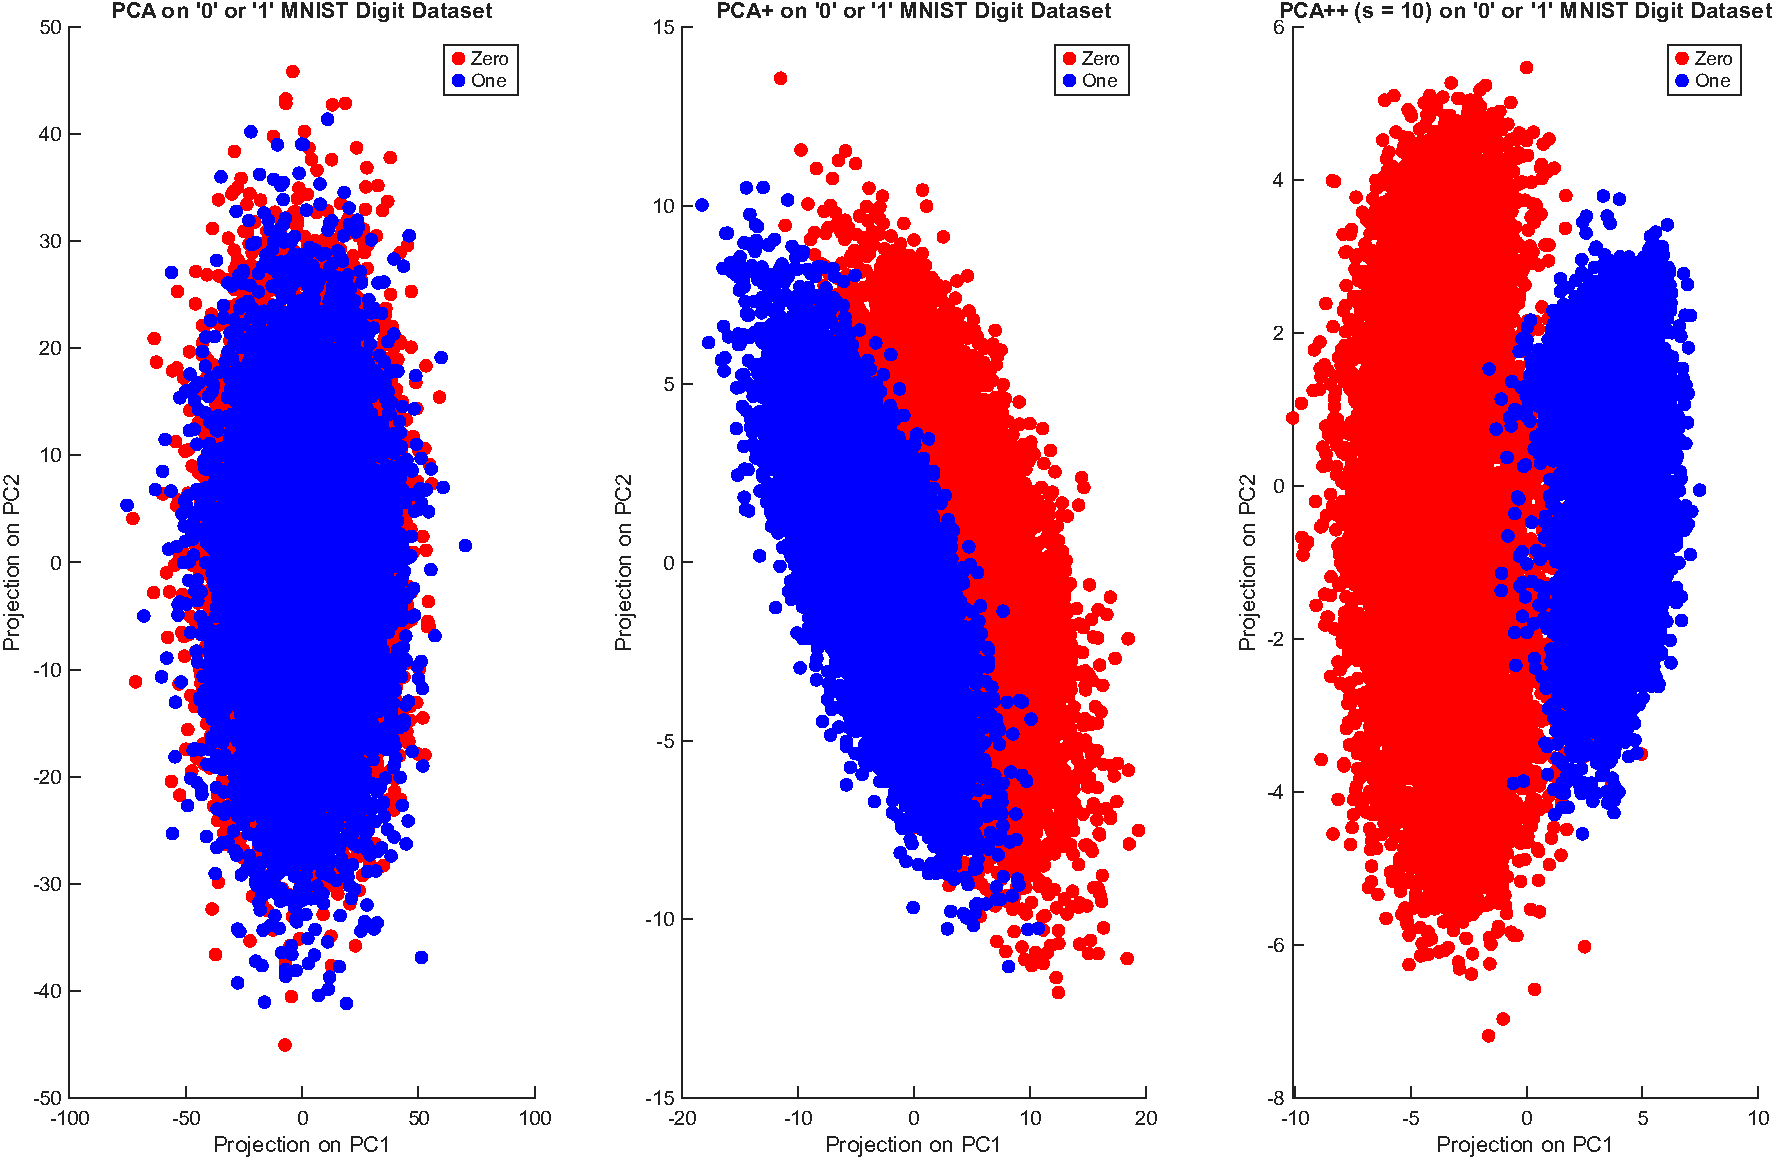
\includegraphics[width=0.8\textwidth]{Figures/MNIST.pdf}
    \caption{\textbf{Left/Middle/Right:} Comparing the performance of PCA/PCA+/PCA++ ($s=10$) in the set of paired MNIST data.}
\label{fig: mnist}
\end{figure}

As expect, figure~\ref{fig: mnist} shows that PCA cannot recover the original signal at all, and we are only left with noise. Meanwhile, PCA+ somewhat manages to differentiate `0' and `1'. Finally, PCA++ is capable of identifying a `0' or a `1' only using the first principal component. This exemplifies PCA++'s strength even when the relative strength of the background noise is high.

\section{Conclusion}
In this end of semester project, we have covered one of the most important tools in data analysis and its key variants. In addition, we have reproduce the main figures present in \cite{wu2025pcauniformityinducesrobustness} which showcase the incredible performance of PCA++ over regular PCA and PCA+. In doing this, I have truly solidified my understanding of PCA as a idea, and as an algorithm.

\newpage

\bibliographystyle{abbrv}
\bibliography{papers}


\newpage

\appendix
\section{Implementation Details}
\section{Attempt at kPCA+} \label{app: kPCA+}
As in the first section, PCA+ remains a linear method that cannot capture nonlinear behaviour correctly. The goal of this section is to apply the kerel approach as in section~\ref{sec: kPCA} to capture this sort of behaviour. We again work under the assumption of paired data $\{(x_n, x_n^+)\}_{n = 1}^{N}$ in $\R^p$ that are composed of a shared signal, independent background signal, and and noise. True to the kernel approach, we consider a nonlinear map $\phi:\R^p \to \R^P$ with $P \ge p$ and apply PCA+ to the augmented data $\{(\phi(x_n), \phi(x_n^+))\}_{n = 1}^{N}$. This means we apply PCA on the matrix
\[
C^+ = \frac{1}{2N} \left( \sum_{n = 1}^{N} \phi(x_n) \phi(x_n^+)^T + \phi(x_n^+) \phi(x_n)^T \right).
\]
Writing the eigenvalue equation, we obtain
\[
\begin{split}
   C^+ b_j = \lambda_j b_j &\iff \left( \sum_{n = 1}^{N} \phi(x_n) \phi(x_n^+)^T + \phi(x_n^+) \phi(x_n)^T \right) b_j = \lambda_j b_j \\
   &\iff \sum_{n = 1}^{N} \phi(x_n) \frac{1}{2N \lambda_j}\phi(x_n^+)^T b_j + \phi(x_n^+) \frac{1}{2N \lambda_j}\phi(x_n)^T b_j = b_j.
\end{split}
\]
Letting
\[
c_{j,n} = \frac{1}{2N \lambda_j}\phi(x_n^+)^T b_j, \quad c^+_{j,n} = \frac{1}{2N \lambda_j}\phi(x_n)^T b_j,
\]
we see that
\[
b_j = \sum_{n = 1}^{N} c_{j,n} \phi(x_n) + c^+_{j,n} \phi(x_n^+).
\]
Returning to the eigen problem and replacing $b_j$ with our new expression, one obtains
\[
\frac{1}{2N} \left( \sum_{n = 1}^{N} \phi(x_n) \phi(x_n^+)^T + \phi(x_n^+) \phi(x_n)^T \right) \sum_{m = 1}^{N} c_{j,m} \phi(x_m) + c^+_{j,m} \phi(x_m^+) = \lambda_j \sum_{n = 1}^{N} c_{j,n} \phi(x_n) + c^+_{j,n} \phi(x_n^+).
\]
We now define 4 kernel matrices $K_{(X)}, K_{X+}, K_{(X,X^+)}, K_{(X^+, X)}$
\[
\begin{split}
    &{K_{(X)}}_{n,m} = \phi(x_n)^T\phi(x_m), \quad {K_{(X^+)}}_{n,m} = \phi(x_n^+)^T\phi(x_m^+), \\
    &{K_{(X,X^+)}}_{n,m} = \phi(x_n)^T\phi(x_m^+), \quad {K_{(X^+, X)}}_{n,m} = \phi(x_n^+)^T\phi(x_m).
\end{split}
\]
After moving the $\frac{1}{2N}$ constant to the right, the left hand side becomes
\[
\begin{split}
  &\sum_{n = 1}^{N} \sum_{m = 1}^{N} \left( \phi(x_n) \phi(x_n^+)^T + \phi(x_n^+) \phi(x_n)^T \right) \left( c_{j,m}\phi(x_m) + c^+_{j,m} \phi(x_m^+) \right) \\
  =& \sum_{n = 1}^{N} \sum_{m = 1}^{N} c_{j,m} \phi(x_n){K_{(X^+, X)}}_{n,m} + c_{j,m} \phi(x_n^+){K_{(X)}}_{n,m} + c^+_{j,m} \phi(x_n){K_{(X^+)}}_{n,m} + c^+_{j,m} \phi(x_n^+){K_{(X,X^+)}}_{n,m} \\
  =& \sum_{n = 1}^{N} \phi(x_n) \sum_{m = 1}^{N} c_{j,m} {K_{(X^+, X)}}_{n,m} + c^+_{j,m}{K_{(X^+)}}_{n,m} + \sum_{n = 1}^{N} \phi(x_n^+) \sum_{m = 1}^{N} c_{j,m} {K_{(X)}}_{n,m} + c^+_{j,m}{K_{(X,X^+)}}_{n,m} \\
  =& \sum_{n = 1}^{N} \phi(x_n) \left( K_{(X^+, X)}c_j + K_{(X^+)}c^+_j \right)_n + \sum_{n=1}^{N} \phi(x_n^+) \left(K_{(X)}c_j + K_{(X,X^+)} c^+_j\right)_n.
\end{split}
\]
Premultiplying this equation by $\phi(x_\ell)^T + \phi(x_\ell^+)^T$, we obtain
\[
\begin{split}
    &\sum_{n = 1}^{N} \left({K_{(X)}}_{\ell, n} + {K_{(X^+, X)}}_{\ell,n}\right) \left(K_{(X^+, X)}c_j + K_{(X^+)}c^+_j\right)_n \\
    +&\sum_{n=1}^{N} \left({K_{(X,X^+)}}_{\ell,n} + {K_{(X^+)}}_{\ell, n}\right) \left(K_{(X)}c_j + K_{(X,X^+)} c^+_j \right)_n, \quad \forall \ell = 1, \dots, N.
\end{split}
\]
In matrix form, this is
\[
\begin{split}
    &\left( K_{(X)}K_{(X^+, X)} + K_{(X^+, X)}^2 + K_{(X,X^+)}K_{(X)} + K_{(X^+)}K_{(X)} \right) c_j \\
    +& \left( K_{(X)}K_{(X^+)} + K_{(X^+, X)}K_{(X^+)} + K_{(X,X^+)}^2 + K_{(X^+)}K_{(X,X^+)}\right)c^+_j.
\end{split}
\]
Doing the same multiplication on the right hand side leads to
\[
2N\lambda_j \sum_{n = 1}^{N} c_{j,n} \left({K_{(X)}}_{\ell, n} + {K_{(X^+,X)}}_{\ell, n}\right) + c^+_{j,n} \left({K_{(X,X^+)}}_{\ell, n} + {K_{(X^+)}}_{\ell, n}\right), \quad \forall \ell = 1, \dots, N.
\]
In matrix form, this is
\[
2N\lambda_j \left( (K_{(X)} + K_{(X^+,X)})c_j + (K_{(X,X^+)} + K_{(X^+)})c^+_j\right).
\]
At this point, barring other assumptions, there is no clever way to progress.

\end{document}
